\documentclass[12pt]{article}
\usepackage[papersize={8cm,12cm},margin={.5cm,.5cm}]{geometry}
\usepackage{common}
\usepackage{amssymb}
\begin{document}
\begin{problem}[widest=10]
  \item[10.] 關於圖(六)中的直角柱,下列敘述何者正確?
  \begin{figure}[ht]
    \centering
    \vspace*{-1ex}
    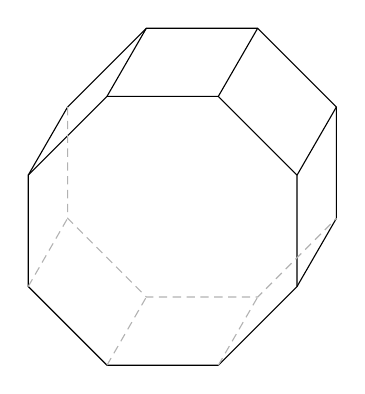
\begin{tikzpicture}
      \draw (-.707,-1.707) -- (.707,-1.707) -- (1.707,-.707) -- (1.707,.707) -- (.707,1.707) -- (-.707,1.707) -- (-1.707,.707) -- (-1.707,-.707) -- (-.707,-1.707);
      \draw[densely dashed,black!30] (-.707,-1.707) -- (-.207,-.841);
      \draw[densely dashed,black!30] (.707,-1.707) -- (1.207,-.841);
      \draw (1.707,-.707) -- (2.207,.159);
      \draw (1.707,.707) -- (2.207,1.573);
      \draw (.707,1.707) -- (1.207,2.573);
      \draw (-.707,1.707) -- (-.207,2.573);
      \draw (-1.707,.707) -- (-1.207,1.573);
      \draw[densely dashed,black!30] (-1.707,-.707) -- (-1.207,.159);
      \draw (2.207,.159) -- (2.207,1.573) -- (1.207,2.573) -- (-.207,2.573) -- (-1.207,1.573);
      \draw[densely dashed,black!30] (-1.207,1.573) -- (-1.207,.159) -- (-.207,-.841) -- (1.207,-.841) -- (2.207,.159);
    \end{tikzpicture}
    \vspace*{-1ex}
    \caption*{圖(六)}
    \vspace*{-2ex}
  \end{figure}
  \begin{choices}
    \item 有 24 個頂點
    \item 有 16 條邊
    \item 有 1 個底面
    \item 有 8 個側面
  \end{choices}
\end{problem}
\end{document}
